\documentclass[]{tukediphc}
%% -----------------------------------------------------------------
%% tento subor ma kodovanie utf-8
%%
%% na kompilaciu pouzivajte format pdfcslatex 
%%
%% vytvorene distribuciou texlive 2009-7, OS GNU/Linux
%% vytvorene distribuciou TeXLive 2010, OS Win XP
%% februar 2013
%% -----------------------------------------------------------------
\usepackage[utf8]{inputenc}
%\usepackage[T1]{fontenc}
\usepackage{lmodern,textcase}
\usepackage[slovak]{babel}\renewcommand{\figurename}{Obr\'azok}
\def\refname{Zoznam pou\v{z}itej literat\'ury}
\usepackage{latexsym}
\usepackage{dcolumn} % zarovnanie cisiel v tabulke podla des. ciarky
\usepackage{hhline}
\usepackage{amsmath}
\usepackage{subfig}
\usepackage{nicefrac} % pekne zlomky
\usepackage{upgreek} % napr. $\upmu\mathrm{m}$ pre mikrometer ...
\usepackage[final]{showkeys}%color%notref%notcite%final
\usepackage[slovak,noprefix]{nomencl}
\makeglossary % prikaz na vytvorenie suboru .glo
\usepackage{parskip}% 'zhusti' polozky obsahu
%%
%\usepackage[dvips]{graphicx}
%\DeclareGraphicsExtensions{.eps}
\usepackage[pdftex]{graphicx}
\DeclareGraphicsExtensions{.pdf,.png,.jpg,.mps}
\graphicspath{{figures/}} % priecinok na obrazky
%%
%% Cislovane citovanie
%\usepackage[numbers]{natbib}
%%
%% Citovanie podľa mena autora a roku
\usepackage{natbib} %\citestyle{chicago}
% -----------------------------------------------------------------
%% tlač !!!
\usepackage[pdftex,unicode=true,bookmarksnumbered=true,
bookmarksopen=true,pdfmenubar=true,pdfview=Fit,linktocpage=true,
pageanchor=true,bookmarkstype=toc,pdfpagemode=UseOutlines,
pdfstartpage=1]{hyperref}
\hypersetup{%
baseurl={http://www.tuke.sk/sevcovic},
pdfcreator={pdfcsLaTeX},
pdfkeywords={Riadenie procesov, Oceliarstvo, Vizualizácia, Virtuálna realita, Matematické modelovanie},
pdftitle={Elaborát z predmetu Riadenie procesov},
pdfauthor={Michal Takáč},
pdfsubject={Dizertačná skúška}
} 
%% nehodiace zakomentujte !
%\dippraca{Elaborát z predmetu Riadenie procesov}
%\bakpraca{Príprava na dizertačnú skúšku}
%%
\nazov{Elaborát z predmetu Riadenie procesov}
%% ked praca nema 'podnazov' zakomentujte nasledujuci riadok
%% alebo polozku nechajte prazdnu
\podnazov{}
\autor{Ing.~Michal Takáč}
\veduciprace{prof.~Ing.~Ivo~Petráš, DrSc.}
\univerzita{Technická univerzita v~Košiciach}
\fakulta{Fakulta baníctva, ekológie, riadenia a geotechnológií}
\skratkafakulty{FBERG}
\katedra{Ústav riadenia a informatizácie výrobných procesov}
\skratkakatedry{URIVP}
\odbor{Riadenie procesov}
\specializacia{Kybernetika}
\abstrakt{Abstrakt je povinnou súčasťou každej práce. Je výstižnou
charakteristikou obsahu dokumentu. Nevyjadruje hodnotiace stanovisko
autora. Má byť\/ taký informatívny, ako to povoľuje podstata práce.
Text abstraktu sa píše ako jeden odstavec. Abstrakt neobsahuje odkazy
na samotný text práce. Mal by mať\/ rozsah 250 až 500 slov. Pri
štylizácii sa používajú celé vety, slovesá v činnom rode a tretej
osobe. Používa sa odborná terminológia, menej zvyčajné termíny,
skratky a~symboly sa pri prvom výskyte v texte definujú.}
\klucoveslova{Riadenie procesov, Oceliarstvo, Vizualizácia, Virtuálna realita, Matematické modelovanie}
\datumodovzdania{12. 5. 2020}
\mesto{Košice}

\begin{document}
\renewcommand\theHfigure{\theHsection.\arabic{figure}}
\renewcommand\theHtable{\theHsection.\arabic{table}}
\bibliographystyle{dcu}

\prvastrana


\thispagestyle{empty}
\tableofcontents
\newpage
%
%\thispagestyle{empty}
%%\addcontentsline{toc}{section}{\numberline{}Zoznam obrázkov}
%\listoffigures
%\newpage
%
%\thispagestyle{empty}
%%\addcontentsline{toc}{section}{\numberline{}Zoznam tabuliek}
%\listoftables
%\newpage

%%%%%%%%%%%%%%%%%%%%%%%%%%%%%%%%%

\setcounter{page}{1}
\setcounter{equation}{0}
\setcounter{figure}{0}
\setcounter{table}{0}

\section{Úvod}

Cieľom riadenia procesu je udržiavať kľúčové parametre prevádzky procesu v úzkom rozmedzí referenčnej hodnoty alebo požadovanej hodnoty. Niekdajšiu potrebu riadiť túto činnosť manuálne v súčasnej dobe nahrádzajú programovateľné automaty a regulátory v snahe ovládať premennú automatizovane. Jednoduchý regulátor môže udržiavať procesnú veličinu v slučke na rovnomernej úrovni, pokiaľ nedôjde k nadmernému rušeniu. Pri komplexných procesoch, ako sú tie v metalurgii, sa využívajú desiatky až stovky takýchto regulátorov, niektoré s integrovanými LCD panelmi \citep{Al-Megren2016}.

Potreba zdokonaľovania a vývoja nových systémov riadenia bola tradične poháňaná požiadavkou presnejšej a nákladovo efektívnejšej výroby. 

Kontrolovať každý z regulátorov jednotlivo si vyžaduje 

%The need for developing improved control systems has traditionally been powered by the demand for more accurate and cost efficient production. This is still a major driving force but environmental issues do also have a profound influence on this development today (\cite{Widlund1998}).

Potreba zdokonaľovania a vývoja nových systémov riadenia bola tradične poháňaná požiadavkou presnejšej a nákladovo efektívnejšej výroby. Je to stále hlavná hnacia sila, no environmentálne otázky majú na tento vývoj zásadný vplyv aj dnes (\cite{Widlund1998}).

Hlavným cieľom riadenia výroby ocele s kyslíkovým konvertorom je získanie predpísaných parametrov ocele, keď sa odoberá z pece, vrátane hmotnosti, teploty a obsahu každého prvku. V procese výroby ocele je kritériom o tom, či je roztavená oceľ prijateľná alebo nie, konečný obsahu uhlíka a teplota taveniny \cite{Wang2010}.

%Generally, the LD/BOF steelmaking process with sub-lance system can be divided into two stages: static control and dynamic control. Static models include oxygen supplying model, slaging model and bottom blowing model; dynamic models include decarburization speed model, molten steel warming model and the model for the amount of coolant. (\cite{Wang2010}).

Všeobecne možno povedať, že riadenie LD procesu (BOF) výroby ocele v LD konvertore s odbernou sondou sa dá rozdeliť do dvoch stupňov: statické riadenie a dynamické riadenie. Statické modely zahŕňajú model prívodu kyslíka, model trosky a model fúkania kyslíka; Medzi dynamické modely patrí model rýchlosti oduhličovania, model otepľovania roztavenej ocele a model množstva chladiacej kvapaliny \cite{Wang2010}.

%The fast dynamics of the LD converter steelmaking process or the BOF process, as it is commonly known, often makes it a challenge to obtain stable blowing conditions and to achieve the required steel composition and temperature simultaneously at the end point. For this reason, process control becomes very necessary and attempts had started as early as in the 1970s (\cite{Fritz2005}). Out of the originally very simple LD process have grown the modern process-controlled and automated production systems that enable present-day adaptations to meet today’s economic and ecological demands (\cite{Sarkar2015}). The non-linear nature of chemical and thermodynamical processes in basic oxygen steelmaking also amassed interest in developing new mathematical models based on fractionalorder calculus.

Rýchla dynamika procesu výroby ocele LD konvertorom sťažuje dosiahnutie stabilných podmienok pre fúkanie kyslíka a súčasne dosiahnutie požadovaného zloženia ocele a teploty v koncovom bode tavenia. Z tohto dôvodu je správne riadenie procesu extrémne dôležité. Prvé pokusy s vývojom systémov automatizovaného riadenia sa začali už v sedemdesiatych rokoch (\cite{Fritz2005}). Z pôvodne veľmi jednoduchého riadenia LD procesu vznikli moderné a automatizované výrobné systémy riadené procesmi, ktoré umožňujú súčasné prispôsobenie sa dnešným hospodárskym a ekologickým požiadavkám (\cite{Sarkar2015}). Nelineárna povaha chemických a termodynamických procesov pri výrobe ocele v LD konvertore tiež vzbudila záujem o vývoj nových matematických modelov založených neceločíselnom diferenciálnom počte.

%\url{https://www.primetals.com/fileadmin/user_upload/content/01_portfolio/2_steelmaking/converter-carbon-steelmaking/Converter_steelmaking_automation.pdf}



\section{Procesy v kyslíkovom konvertore}

Kyslíkový konvertor alebo v niektorých oblastiach sveta nazývaný aj základná kyslíková pec (basic oxygen furnace - BOF) pozostáva z radu komplexných procesov s nebezpečnými vlastnosťami, napríklad z dôvodu vysokej teploty, prachu a vibrácií. V konvertore prebieha  množstvo chemických reakcií a fyzikálnych javov, medzi ktorými sa nájdu aj také, ktorým úplne nerozumieme z dôvodu ich komplexnosti.

Podstatou výroby ocele v kyslíkovom konvertore je oxidácia prvkov z kovonosnej vsádzky s kyslíkom fúkaným do konvertora. Oxidy týchto prvkov prechádzajú do trosky alebo odchádzajú vo forme konvertorového plynu. LD proces sa skladá z~nasledujúcich elementárnych procesov:

\begin{enumerate}
	\item Vsádzanie šrotu
	\item Nalievanie tekutého surového železa
	\item Fúkanie kyslíka a pridávanie troskotvorných a legujúcich prísad
	\item Meranie teploty a zloženia ocele
	\item Odpich ocele
	\item Odpich trosky
\end{enumerate}

V moderných oceliarňach sa vyrobí cca 300t ocele v priebehu 30-40 minútového cyklu. Pre prispôsobenie akosti ocele a tvorbu trosky sa počas pochodu pridávajú rozličné prísady. Počas vsádzania a odpichu je konvertorová pec naklonená. Počas fúkania kyslíka má konvertor zvislú polohu. Zmeny polohy konvertora počas jednotlivých elementárnych procesov sú znázornené na obrázku \ref{o:30}.

\begin{figure}[h!]
	\centering
	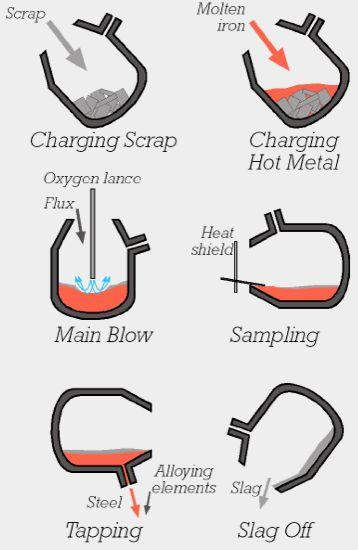
\includegraphics[width=.35\textwidth,angle=0]{convertor-phases.jpg}
	\caption{Znázornenie elementárnych procesov v LD konvertore.}
	\label{o:30}
\end{figure}

V závislosti od miestnych prevádzkových podmienok, dostupnosti šrotu, vysokopecného železa a rozsahu predúpravy, je kovová vsádzka do konvertora (LD/BOF, Q-BOP) tvorená 75 až 95 \% surovým železom a zvyšok je oceľový šrot. Používané druhy šrotu sú zvyčajne tie, ktoré sa vyrábajú v oceliarni: šrot z plechu, poškodené formy, plechovky a podobne \cite{Turkdogan1996}.

Kyslík je fúkaný vysokou rýchlosťou (až do dvojnásobnej rýchlosti zvuku) na povrch kovového kúpeľa v konvertore a v oblasti povrchu sa vytvára tzv. horúce miesto, kde prúd kyslíka naráža na povrch. Oxidačné produkty sa rozpustia v troske s výnimkou oxidu uhoľnatého, ktorý prechádza vrstvou trosky a tvorí hlavnú zložku konvertovaného plynu. Intenzita oxidácie jednotlivých prvkov závisí od ich chemickej afinity ku kyslíku. Oxidácia uhlíka je jedným z najdôležitejších procesov.

\section{Riadenie procesov v kyslíkovom konvertore}

Keďže cieľom výroby ocele v kyslíkových konvertoroch je spálenie (tzv. oxidácia) nežiadúcich nečistôt obsiahnutých v kovovej vsádzke, účelom tohto oxidačného procesu teda je:

\begin{itemize}
	\item znížiť obsah uhlíka na predpísanú úroveň (z približne 4 \% na menej ako 1 \%, ale často nižšie),
	\item upraviť obsah potrebných cudzích prvkov,
	\item odstrániť nežiadúce nečistoty v maximálne možnej miere.
\end{itemize}

Následnou úlohou riadiaceho procesu je potom získanie predpísaných parametrov ocele, ktorá sa odpichuje z konvertora, vrátane hmotnosti, teploty a obsahu každého prvku. Na základe týchto parametrov sa rozhoduje o tom, či je roztavená oceľ prijateľná alebo nie.

Statický model riadenia je založený na celkovej materiálovej bilancii (Fe, troska, kyslík) a celkového tepla. Na základe prepočtov bilancií potom dostaneme informáciu o tom, koľko železnej rudy je potrebné pridať a aký objem kyslíka sa má dofúkať, spolu s konečnou hmotnosťou tekutej ocele a trosky pre dané hmotnosti, zloženie horúceho kovu a zloženie šrotu. Kvôli možnému vzniku chýb z dôvodu nerovnomernosti bilancie hmoty a tepla alebo neznámej časti týchto bilancií je tento model založený na spätnoväzobnom riadení.

Dynamický model riadenia sa zameriava na dynamickú hmotnostnú bilanciu kyslíka, uhlíka a dusíka v spojení s množstvom prietoku a zloženia odpadového plynu. Modely dynamického riadenia sú najčastejšie založené na informáciách o odpadových plynoch a majú schopnosť predvídať stav procesu (zloženie ocele a trosky, ich hmotnosť, teplota) v akomkoľvek okamihu počas procesu.

Počítačom podporované výpočty vsádzky sa robia pre každú tavbu. Asi 80 percent modelu riadenia vsádzky je založený na rovnováhe tepla a materiálu, zvyšok je založený na empirických vzťahoch, ktoré sa medzi jednotlivými taviarňami líšia. Pretože každá oceliareň má svoju vlastnú formuláciu modelu riadenia vsádzky \cite{Turkdogan1996}.

Za účelom monitorovania a riadenia procesu je možné použiť rôzne meracie systémy na poskytnutie spätnej väzby operátorovi alebo priamo existujúcemu systému na automatizované riadenie. Tieto merania môžu byť priame alebo nepriame, ako aj~s~časovým oneskorením alebo bez neho \cite{Widlund1998}.

\begin{figure}[h!]
	\centering
	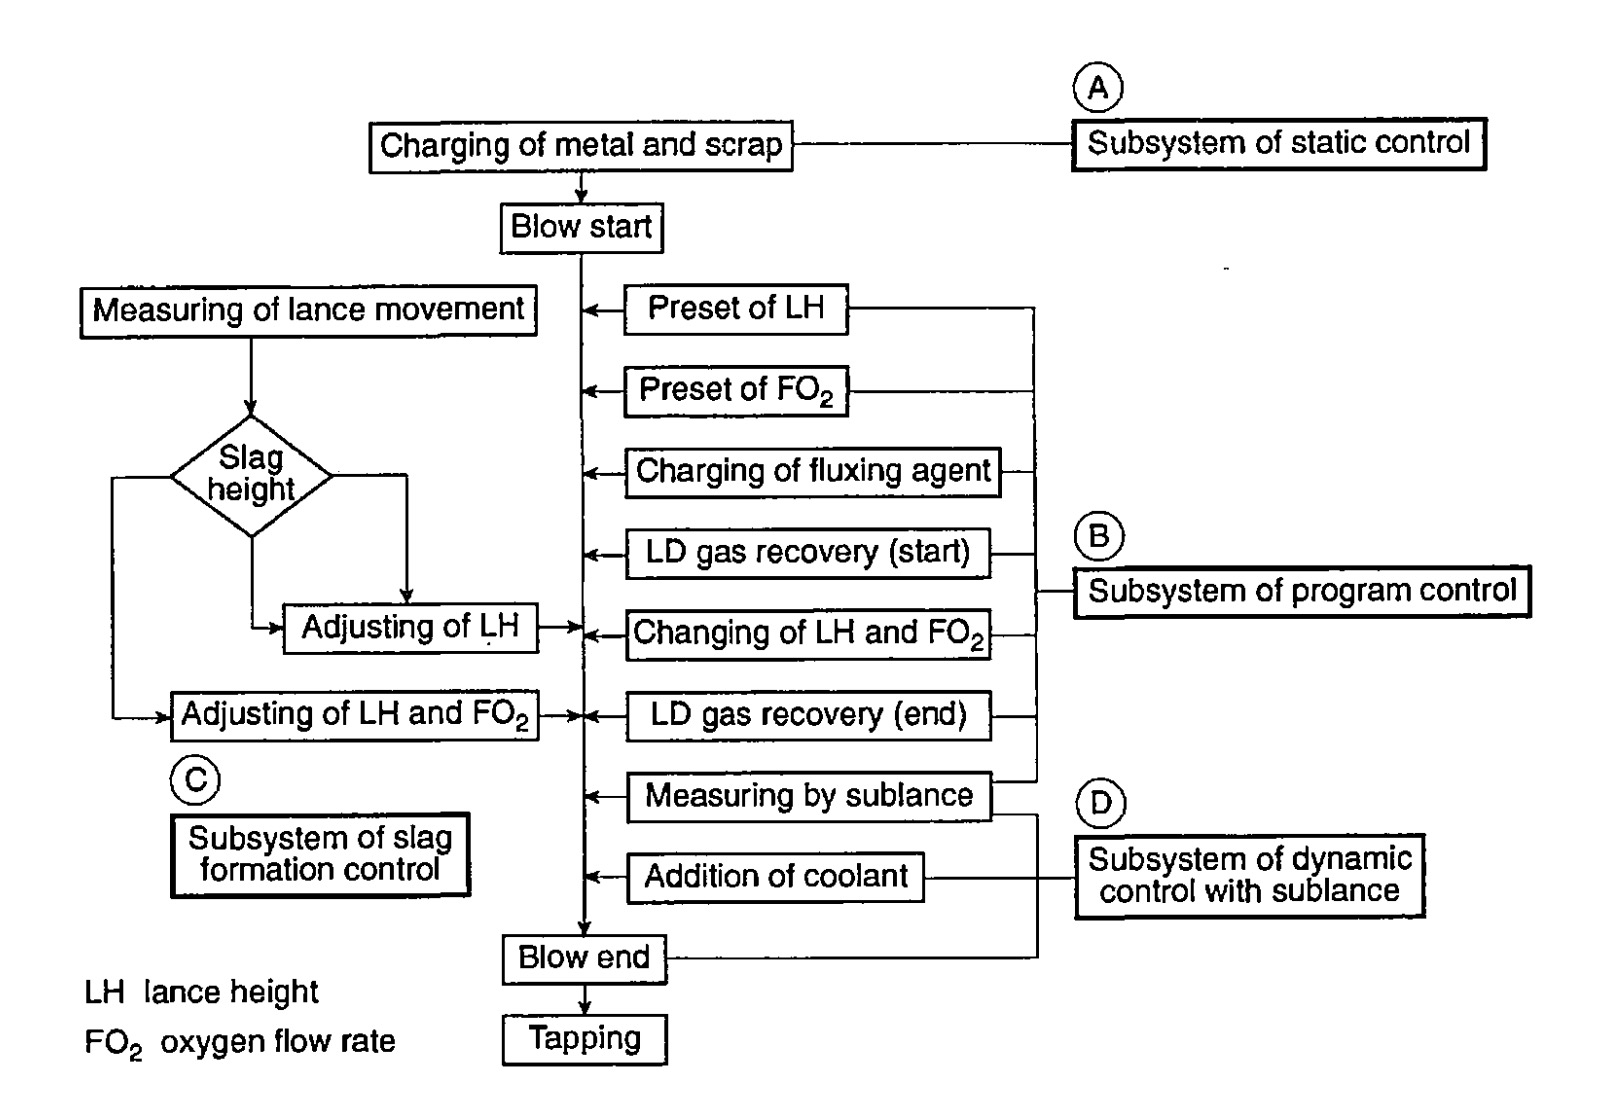
\includegraphics[width=.9\textwidth,angle=0]{figures/schematic-bof.jpg}
	\caption{Schéma funkcionality systému automatizovaného LD procesu \citep{Turkdogan1996}.}
	\label{o:21}
\end{figure}

Existuje len niekoľko procesných premenných, ktoré môže nastavovať riadiaci systém alebo obsluha - výška trysky pre prívod fúkaného kyslíka, prietok kyslíka a~prietok čistiaceho plynu. Zmeny výšky prívodnej trysky sa merajú a nastavujú ľahšie, a preto je lepšie ich používať v riadiacom systéme s uzavretou slučkou. Zmena prietoku kyslíka počas LD procesu nesmie byť väčšia ako 5\%, pretože dýza je navrhnutá pre špecifický prietok \cite{Widlund1998}.

\section{Automatizované riadenie}

Plne optimalizovaná automatizácia riadiacich systémov je základom pre spoľahlivé výrobné procesy, maximálny výkon zariadenia a kvalitné výrobky, ktoré vyhovujú všetkým požiadavkám trhu. V súčasnosti si môžeme všimnúť posun priemyslu do novej paradigmy označovanej ako Priemysel 4.0, dôsledkom ktorej rastie počet podnikov, ktoré implementáciou inteligentných technológií zefektívňujú svoje procesy a znižujú náklady. Postupne sa na túto dráhu tzv. inteligentných výrobných podnikov dostávajú aj taviarne. Pece sú vybavené stále väčším počtom senzorov, digitálne modely zvyšujú stupeň automatizácie a informácie sú zdieľané medzi rôznymi agregátmi v rámci
rastlina


Systémy optimalizácie procesov zahŕňajú pokročilé procesné modely, využitie umelej inteligencie, grafické užívateľské rozhrania pre manuálne riadenie procesov človekom (SCADA, HMI, vizualizácie dát) a prevádzkové odborné znalosti. Procesné modely optimalizujú rôzne výrobné procesy so zreteľom na zníženie spotreby energie a emisií.

Automatizácia

Základnú časť automatizácie LD procesu


Naklápací pohon kovertora

Úlohou naklápacích pohonov je rotácia nádoby konvertora do plniacej, vyprázdňovacej alebo vzorkovacej polohy.

Systém s uzavretou slučkou (closed-loop)



Miešanie zdola - ovládanie jedným vedením
Riadiaci systém kyslíkovej dýzy

\subsection{Odoberanie vzoriek taveniny a meranie teploty}

Odberná sonda je dôležitým nástrojom pri výrobe ocele LD procesom. Poskytuje operátorovi cenné informácie o procese tavby akými sú teplota taveniny a jej zloženie. kým je teleso konvertora v zvislej polohe. Zavádza sa automatizovane do vnútra konvertora cez bočný otvor kým je teleso konvertora v zvislej polohe, a to 2-krát počas tavby bez nutnosti jej prerušenia. Prvé zavedenie sondy zväčša býva po vyfúkaní 90\% objemu kyslíka vyčleneného pre danú tavbu, kedy sa meria teplota, objem uhlíka, zloženie trosky, výška oceľového kúpeľa a úrovne trosky. Druhé zavedenie sa uskutočňuje po procese fúkania.

\begin{figure}[!ht]
	\centering
	\subfloat[Odberná sonda od Berry Metal Company.]{{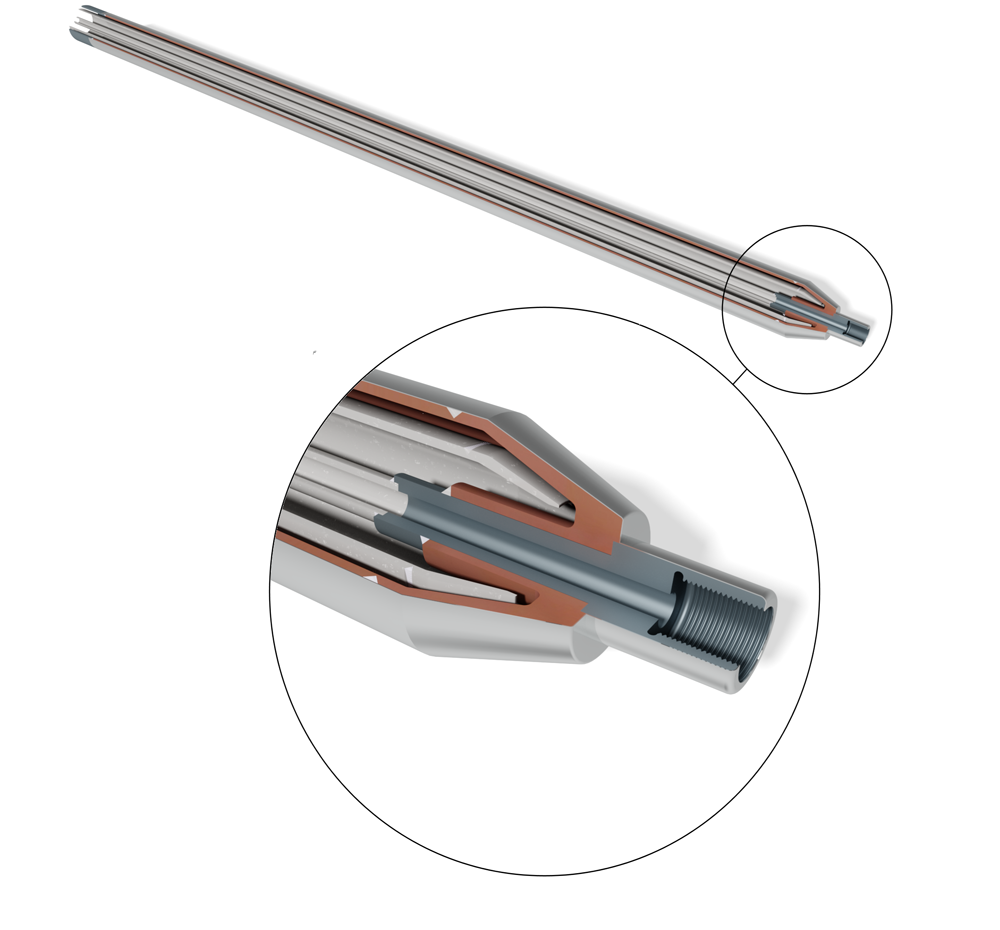
\includegraphics[width=6.5cm]{figures/sub-lance-berry.png} }}%
	\qquad
	\subfloat[Odber vzorky taveniny odbernou sondou v praxi.]{{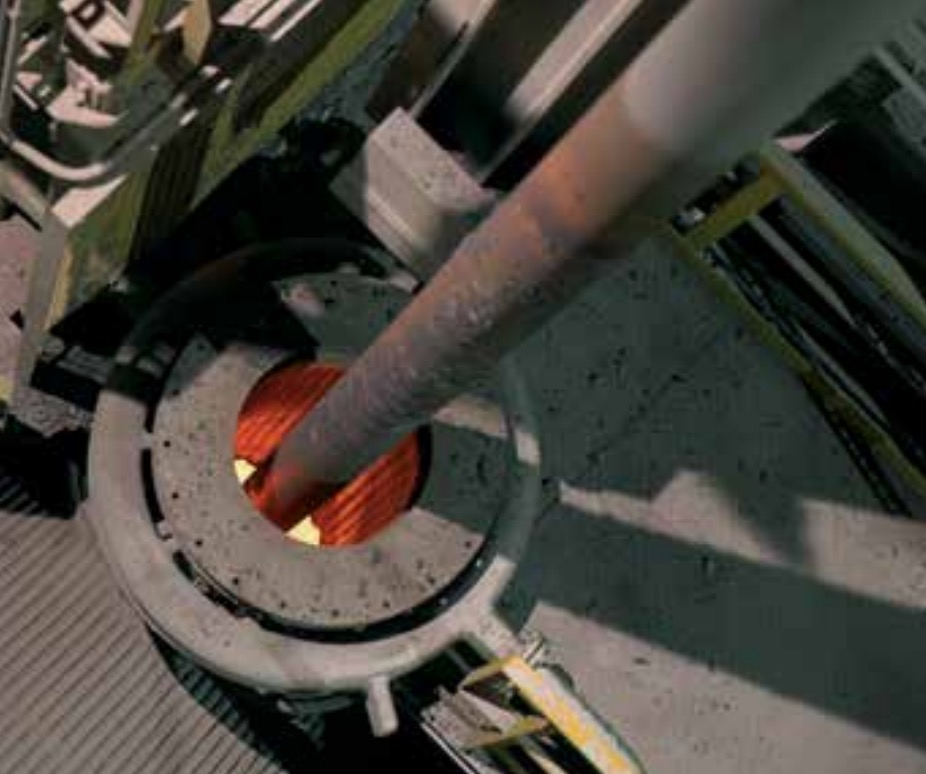
\includegraphics[width=7.35cm]{figures/sublance.jpg} }}
	\caption{Odberná sonda.}
	\label{o:21}
\end{figure}

Moderné konvertory prevádzkujú merania odbernými sondami v spojení s kombinovaným statickým a dynamickým modelom riadenia procesu (SDM).
Informácie získané z odbernej sondy sú ďalej spracované riadiacim systémom, ktorého optimalizačný model sa snaží dosiahnúť optimálne 

Horizontálny merací manipulátor
Automatický odpichový systém
Pneumatická zarážka trosky
Manipulácia s materiálom
Váženie a kontrola prísad a zliatin
Chladenie a čistenie odpadového plynu
Zhodnotenie a analýza plynu
Blokovací a poplachový systém



%
%%
\Urlmuskip=0mu plus 1mu\relax
\bibliographystyle{spbasic}
\bibliography{refs/control,refs/mathematics,refs/modeling,refs/cfd,refs/lbm,refs/gpu,refs/interaction,refs/interfaces,refs/hci,refs/design,refs/ml,refs/visualization,refs/programming,refs/simulation,refs/ar,refs/vr,refs/online}

%

\end{document}
%%